\documentclass[output=paper,colorlinks,citecolor=brown,
% hidelinks,
% showindex
]{langscibook}

\author{Damien Fleury\affiliation{University of Paris} and Lucia M. Tovena\affiliation{Universit\'e de Paris}}
\todo[inline]{Standardize university name?}
\title{On the pragmasemantics of a high adjunct wh-word}
\abstract{
Questions with \textit{comment} (how) in French may allow a reason reading when they occur in sentence initial position, besides manner and means reading.  The paper provides empirical evidence in support of an analysis of this type of \textit{comment} as externally merged in the left periphery of the clause, adapting existing proposals for reason `why' counterparts. These questions convey the information that the proposition about the described situation, hereafter the prejacent, disconfirms the speaker's expectations. They express her attempt to get information to resolve this conflict. \textit{Comment} signals this particular function of the question and works as a discourse management device that aims to align the viewpoints of the interlocutors about preconditions to admitting the prejacent into the common ground.
}

\IfFileExists{../localcommands.tex}{%hack to check whether this is being compiled as part of a collection or standalone
   % add all extra packages you need to load to this file

\usepackage{tabularx,multicol,multirow}
\usepackage{url}
\urlstyle{same}

\usepackage{listings}
\lstset{basicstyle=\ttfamily,tabsize=2,breaklines=true}

\usepackage{langsci-basic}
\usepackage{langsci-optional}
\usepackage{langsci-lgr}
\usepackage{langsci-gb4e}
%    \let\eachwordone=\it % Ch 14, 18

\usepackage{jambox}
\usepackage{subfigure}
\usepackage{tablefootnote}
\usepackage[nameinlink, noabbrev]{cleveref}
\crefname{enumi}{example}{examples}

\usepackage{bbding}
%\usepackage{linguex}
\usepackage{stmaryrd}

\usepackage{tipa}
\let\ipa\textipa
\usepackage{vowel}
\newcommand{\BlankCell}{}
\usepackage{ot-tableau}

\usepackage{forest}
\useforestlibrary{linguistics}
\usepackage[noeepic]{qtree}
\usepackage{pstricks, pst-xkey, pst-jtree}
\usepackage{tikz-qtree}
\usepackage{tikz-qtree-compat}
\usepackage{tree-dvips}

\usepackage{lastpage}
\usepackage{hyperref}
\usepackage{xltxtra}

\usepackage{ragged2e}
%\usepackage{subcaption}
\usepackage{floatrow}
\usepackage{float}

\usepackage[normalem]{ulem} % Pour les textes barrés
\usepackage{ifthen} 

\usepackage{todonotes}

   \newcommand*{\orcid}{}

\makeatletter
\let\theauthor\@author
\makeatother

\papernote{\scriptsize\normalfont
    \theauthor.
    \titleTemp. 
    To appear in: 
    Chad Howe and Pilar Chamorro and Timothy Gupton and Margaret Renwick.
    Theory, Data, and Practice: Selected papers from the 49th Linguistic Symposium on Romance Language
    Berlin: Language Science Press. [preliminary page numbering]
}

% Workaround for subscripts with capital letters
\newcommand{\capsub}[1]{\ensuremath{_\text{#1}}}

% Chapter 10: Table-like presentation within example environment
% classical latin > {*}late latin > old french  earlier > later   gloss
\newcommand{\montanoboxi}[7]{\parbox{2cm}{#1} > {#2}\parbox{2cm}{#3} > \parbox{1.5cm}{\textit{#4}} \parbox{1.2cm}{#5}\ > \parbox{1.2cm}{#6} \parbox{1.5cm}{#7}}
% {*}latin > earlier OF [ipa] > early OF   gloss
\newcommand{\montanoboxii}[6]{{#1}\parbox{1.9cm}{\textit{#2}} > \parbox{1.3cm}{\textit{#3}} \parbox{2cm}{#4} \parbox{2cm}{#5} \parbox{1.9cm}{#6}}

% Chapter 5
\newcommand{\redc}[1]{\textcolor{red}{#1}}
\newcommand{\bluec}[1]{\textcolor{blue}{#1}}
\newcommand{\ajout}[1]{\textcolor{blue}{#1}}
\newcommand{\ajoutplus}[1]{\textcolor{cyan}{#1}}

\newcommand{\hachure}[9]{
% Parametres :
% Coordonnees bas gauche (2 parametres) : (#1,#2)
% Coordonnees haut droit (2 parametres) : (#3,#4)
% Orientation : #5
%   1 : diagonale de pente 1
%  -1 : diagonale de pente -1
%   0 : horizontal
%   2 : vertical
% Nombre de pas horizontaux : #6
% Epaisseur du trait : #7
% Couleur : #8 (ex. green)
% Atténuation couleur : #9 (ex. 30)
\pgfmathsetmacro{\N}{#6-1}
\pgfmathsetmacro{\A}{#1}
\pgfmathsetmacro{\B}{#2}
\pgfmathsetmacro{\C}{#3}
\pgfmathsetmacro{\D}{#4}
\pgfmathsetmacro{\I}{(#3-#1)/#6}
\pgfmathsetmacro{\J}{(#4-#2)/#6}
\ifthenelse{\equal{#5}{1}}{
  \foreach \n in {0,...,\N}
    \foreach \m in {0,...,\N}
      {
        \pgfmathsetmacro{\X}{\A + ((0 + \n) * \I)}
        \pgfmathsetmacro{\Y}{\B + ((0 + \m) * \J)}
        \pgfmathsetmacro{\U}{\A + ((1 + \n) * \I)}
        \pgfmathsetmacro{\V}{\B + ((1 + \m) * \J)}
        \draw[#8!#9,#7] (\X, \Y)--(\U, \V);
      } 
  }{}
\ifthenelse{\equal{#5}{-1}}{
  \foreach \n in {0,...,\N}
    \foreach \m in {0,...,\N}
      {
        \pgfmathsetmacro{\X}{\A + ((1 + \n) * \I)}
        \pgfmathsetmacro{\Y}{\B + ((0 + \m) * \J)}
        \pgfmathsetmacro{\U}{\A + ((0 + \n) * \I)}
        \pgfmathsetmacro{\V}{\B + ((1 + \m) * \J)}
        \draw[#8!#9,#7] (\X, \Y)--(\U, \V);
      } 
  }{}
\ifthenelse{\equal{#5}{0}}{
  \foreach \n in {0,...,\N}
    \foreach \m in {0,...,\N}
      {
        \pgfmathsetmacro{\X}{\A + ((0 + \n) * \I)}
        \pgfmathsetmacro{\Y}{\B + ((0 + \m) * \J)}
        \pgfmathsetmacro{\U}{\A + ((1 + \n) * \I)}
        \pgfmathsetmacro{\V}{\B + ((0 + \m) * \J)}
        \draw[#8!#9,#7] (\X, \Y)--(\U, \V);
      } 
  }{}
\ifthenelse{\equal{#5}{2}}{
  \foreach \n in {0,...,\N}
    \foreach \m in {0,...,\N}
      {
        \pgfmathsetmacro{\X}{\A + ((0 + \n) * \I)}
        \pgfmathsetmacro{\Y}{\B + ((0 + \m) * \J)}
        \pgfmathsetmacro{\U}{\A + ((0 + \n) * \I)}
        \pgfmathsetmacro{\V}{\B + ((1 + \m) * \J)}
        \draw[#8!#9,#7] (\X, \Y)--(\U, \V);
      } 
  }{}
}

%Définition d'un pattern de type hachure
% \usetikzlibrary{patterns}
% \makeatletter
% \tikzset{hatch distance/.store in=\hatchdistance,hatch distance=5pt,hatch thickness/.store in=\hatchthickness,hatch thickness=5pt}

% \pgfdeclarepatternformonly[\hatchdistance,\hatchthickness]{north east hatch}% name
%     {\pgfqpoint{-\hatchthickness}{-\hatchthickness}}% below left
%     {\pgfqpoint{\hatchdistance+\hatchthickness}{\hatchdistance+\hatchthickness}}% above right
%     {\pgfpoint{\hatchdistance}{\hatchdistance}}%
%     {
%         \pgfsetcolor{\tikz@pattern@color}
%         \pgfsetlinewidth{\hatchthickness}
%         \pgfpathmoveto{\pgfqpoint{-\hatchthickness}{-\hatchthickness}}       
%         \pgfpathlineto{\pgfqpoint{\hatchdistance+\hatchthickness}{\hatchdistance+\hatchthickness}}
%         \pgfusepath{stroke}
%     }
% \pgfdeclarepatternformonly[\hatchdistance,\hatchthickness]{north west hatch}% name
%     {\pgfqpoint{-\hatchthickness}{-\hatchthickness}}% below left
%     {\pgfqpoint{\hatchdistance+\hatchthickness}{\hatchdistance+\hatchthickness}}% above right
%     {\pgfpoint{\hatchdistance}{\hatchdistance}}%
%     {
%         \pgfsetcolor{\tikz@pattern@color}
%         \pgfsetlinewidth{\hatchthickness}
%         \pgfpathmoveto{\pgfqpoint{\hatchdistance+\hatchthickness}{-\hatchthickness}}
%         \pgfpathlineto{\pgfqpoint{-\hatchthickness}{\hatchdistance+\hatchthickness}}
%         \pgfusepath{stroke}
%     }
% \makeatother
%~~~~~~~~~~~~~~~~~~~~~~~~~~~~~~~~~~~~~


% Chapter 7
\newcommand\pef[1]{(\ref{#1})}

\newcommand{\subscript}[1]{\textsubscript}

   %% hyphenation points for line breaks
%% Normally, automatic hyphenation in LaTeX is very good
%% If a word is mis-hyphenated, add it to this file
%%
%% add information to TeX file before \begin{document} with:
%% %% hyphenation points for line breaks
%% Normally, automatic hyphenation in LaTeX is very good
%% If a word is mis-hyphenated, add it to this file
%%
%% add information to TeX file before \begin{document} with:
%% %% hyphenation points for line breaks
%% Normally, automatic hyphenation in LaTeX is very good
%% If a word is mis-hyphenated, add it to this file
%%
%% add information to TeX file before \begin{document} with:
%% \include{localhyphenation}
\hyphenation{
anaph-o-ra
Dor-drecht
%FFI2016-76045-P-AEI/-MINEICO/-FEDE
}

\hyphenation{
anaph-o-ra
Dor-drecht
%FFI2016-76045-P-AEI/-MINEICO/-FEDE
}

\hyphenation{
anaph-o-ra
Dor-drecht
%FFI2016-76045-P-AEI/-MINEICO/-FEDE
}

    \bibliography{localbibliography}
    \togglepaper[23]
}{}

\begin{document}
\maketitle


\section{Issues about reason-\textit{comment} (how)}\label{intro}
%%%%%%%%%%%%%%%%%%%%%%%%%%%%%%%%%%%%%%%%%%%%%%%%%%%%%%%%%%%%%%%%%%%%%%%%%%%%%%

\subsection{When \textit{comment} (how) is asking about reasons}

The `canonical' interpretation of  \textit{comment} (how) in French is as a wh-item that allows one to question about manners and means, see   (\ref{ex:fleury:1ma-a}) and (\ref{ex:fleury:1ma-b}) respectively.\footnote{The abbreviations used in this paper are glossed as follows: Cl: clitic personal pronoun; \textsc{cond}: conditional mood; \textsc{dat}: dative case; Neg: negation marker; \textsc{t}-: epenthetic `t' consonant.}
Moreover, questions with \textit{comment} such as  (\ref{ex:fleury:1}), 
allow a {reason reading}, highlighted by the possible congruent answer   (\ref{ex:fleury:1b}).
Possible answers with the manner and means readings
are still available, but less salient in this context.\footnote{According to \cite{Cysouw04}, the interrogative category of `manner' is only lexicalised in about 40\% of the world's languages. In many of these, wh-words or expressions with this meaning can form questions with reason flavoured readings. These questions differ in their pragmatic content, and a characteristics of reason-\textit{comment} questions is that they convey the information that the prejacent disconfirms the speaker's expectations. Reason readings are available when the wh-words occur in the highest layer of the structure of the sentence, a.o. see \citep{Rizzi01,Ko05,Tsai08}. How these readings relate to manner and what is their affinity with modality are research issues beyond the scope of this paper.}

\begin{exe}
\ex\label{ex:fleury:1ma} \gll  Comment Daniel tourne-t-il cette plaque\,?  \\
  how Daniel turn-\textsc{t}-he this plate  \\
\glt   How does Daniel turn this plate?
\begin{xlist}
\ex\label{ex:fleury:1ma-a}
\gll Lentement\\
Slowly\\\jambox{(manner)}
\ex \label{ex:fleury:1ma-b}
\gll Avec un tournevis \\ 
With a screwdriver.\\\jambox{(means)}
\end{xlist}
\end{exe}

\begin{exe}
\ex\label{ex:fleury:1} 
\gll Q:  Comment Max peut-il lire le courrier de Paul\,?  \\   
{~} how Max can-he read the mail of Paul \\ 
\glt {~~~~} How can Max read Paul's mail? 
\begin{xlist}
\ex \label{ex:fleury:1a} 
A: Il est curieux.\\
He is nosy.\jambox{(reason)}
\ex \label{ex:fleury:1b}
A: A la h\^ate\\
\glt Cursorily\\
\ex \label{ex:fleury:1c}
A: Avec une loupe\\
With a hand magnifier\\
\end{xlist}
\end{exe}

Question (\ref{ex:fleury:1}), under its reason reading,   has the form of a wh question, but
is not a `standard' constituent question at least insofar as the wh-item is understood not to bind a variable within the {IP} syntactic structure. Neither is it  a yes/no question, for that matter, and cannot receive a yes/no answer. 
The question is about the reasons the event of `Max reading Paul's mail' could come about. 
It is an inquiry about elements of (possibly private)  explanatory theories that would support  some data. 
Such data, which can be contextually available,
%\sout{is}
%\ajout{
are
%}
recalled in the question by 
  the proposition expressed by the clause that would correspond to the sentence radical in the manner and reason readings were it not for the absence of a gap in the IP. Here, the sentence radical is saturated, if we can say so when comparing this questions with others about adjuncts, {and is interpreted as a proposition, not as a propositional function}. Such a proposition is referred to as `prejacent' hereafter. 
 The  {prejacent} in sentence  (\ref{ex:fleury:1}) is the proposition `Max lit le courrier de Paul'.
 

Another specificity of questions like (\ref{ex:fleury:1}) is that they show some characteristics usually associated with exclamation and mirativity, though the intonation is not typical of exclamatives.
Namely, they typically convey the information that the 
situation described by the prejacent disconfirms the speaker's expectations.
At times, they may carry a hint of disapproval, or
have a rhetorical flavour. 



%%%%%%%%%%%%%%%%%%%%%%%%%%%%%%%%%%%%%%%%%%%%%%%%%%%%%%%%%%%%%%%%%%%%%%%%%%%%%%
\subsection{Some strands of analysis}\label{strands}

The reason reading of  \textit{comment}  in question (\ref{ex:fleury:1}) concerns the reasons the situation of `Max reading Paul's mail' could come about, as just noted. This reading makes \textit{comment}  somewhat close to `why', and is reminiscent of the why-how alternation discussed by \citep{Collins91,Ochi04,Tsai08}
among others. 
It is worth underscoring that the cases of why-how alternation discussed in the literature  seem to relate to the reason readings of these two wh-items, not to the wh-items in themselves. 
%
As an aside, it should also be noted that \textit{comment} questions differ from these cases of alternation because the prejacent describes a situation that is not necessarily true, as it may be potential or actual. Therefore, it is not presupposed,
although this might not appear from the English translations. Factors  enhancing the factuality of the prejacent are e.g.\  the use of  the pass\'e compos\'e in the clause, as illustrated by (\ref{ex:fleury:2}).
Factors going against it are e.g.\ the use of a conditional verb form, as illustrated by (\ref{ex:fleury:3}). In all cases, the prejacent conveys at issue information, and the reason(s) for the (potential) actualisation of the situation it describes are focussed on in the question. 

\begin{exe}
\ex\label{ex:fleury:2} 
\gll Comment Max a lu le courrier de Paul\,? \\
how Max has read the mail of Paul \\
\glt How comes that Max read Paul's mail?
\ex\label{ex:fleury:3} 
\gll Comment Max aurait lu le courrier de Paul\,? \\
how Max have.\textsc{cond} read the mail of Paul \\
\glt How could it be that Max read Paul's mail?
\end{exe}



Reason questions can also be worded with \textit{pourquoi} (why)  in French, see (\ref{pp0}). 
Indeed,  \textit{pourquoi} can be replaced by \textit{comment} in cases such as (\ref{pp0}), when the question is used to inquire about the conditions that led to formulating the request for a deadline. 
\begin{exe}
\ex \label{pp0} \gll Pourquoi il doit te r\'epondre avant mardi\,? \\
why he must you-\textsc{dat} answer before Tuesday \\
\glt Why should he answer to you by Tuesday?
\end{exe}
However,  \textit{pourquoi} does not alternate with   \textit{comment}  when used for inquiring about  the goal/purpose  of the initiator of the event, or the situation that would ensue (result). 
%\ajout{
The example in (\ref{ex:fleury:HowPolice1}) presents a wh-question that is acceptable and has a reason interpretation with either wh-word. However, only the version with \textit{pourquoi} is compatible with the continuation given in (\ref{ex:fleury:HowPolice3}), as indicated with the diacritic `\#/${ok}$'.
\begin{exe}
\ex \label{ex:fleury:HowPolice0}
\begin{xlist}
\ex \label{ex:fleury:HowPolice1} \gll Comment/pourquoi {l'agent de police} tol\`ere-t-il un tel d\'esordre\,?\\
how/why the-police-officer allow-\textsc{t}-he a such mess \\
\glt How come/why the police officer allows such a mess?
\ex \label{ex:fleury:HowPolice3} \gll \#/${ok}$  Pour \'eviter une confrontation inutile\\
{} to avoid a confrontation unnecessary\\
\glt In order to avoid unnecessary confrontation.
\end{xlist}
\end{exe} 


As we said, \textit{comment\/}   interpreted as inquiring about a reason occurs in sentence initial position, where it is  understood not to bind a variable low in the syntactic structure, below the IP node. 
%
The semantic intuition that \textit{comment} works as operating over  the rest of the sentence from outside the clause,   questioning some conditions about the prejacent  $p$,  can be substantiated by extending to this case syntactic proposals put forth for reason \textit{why}.
In the literature, it has been argued that the adjunct \textit{why}  in questions like \textit{Why did Max leave?} is externally merged in the left periphery of the clause and does not bind any syntactic variable inside the IP, cf.\/ \citep{Rizzi90, Rizzi01}, \citep{ShlonskySoare11} among others. %\ajout{o.a.}
A similar 
analysis may be explored for \textit{comment} with a reason reading in  (\ref{ex:fleury:1}).
%, 
In \sectref{sec:fleury:high}, we provide empirical support for it. 
An expected advantage is that the reason reading of the two wh-expressions \textit{comment} and \textit{why}  would receive a similar  characterisation that is compatible with
the discourse role of the prejacent.


Next, as we mentioned above,  reason-\textit{comment} questions show some characteristics usually associated with exclamation and mirativity.
Surprise can be conveyed by other linguistic expressions in French, whose use, in turn, 
is not limited to the expression of surprise, e.g. wh-exclamatives (\ref{pp1}).
\begin{exe}
\ex \label{pp1} \gll Qu'est-ce qu'il est grand\,! \\
what-is-it that-he is tall\\
\glt How tall is he!
\end{exe}

The characterisation of reason-\textit{comment} that we suggest partially overlaps analyses of exclamatives and mirativity, insofar as we
assume that reason-\textit{comment} operates on speaker's expectations.
%
We assume that in asking a \textit{comment} question with a reason reading, the speaker initiates  an {attributional search}  in reaction to an expectation disconfirmation, following \cite{FleuryTovena18}. 
 In social psychology, {attributions} \citep{Heider58} are the explanations humans come up with in order to understand the causes of behaviours, actions and events.    The search verbalised with a \textit{comment} question aims at finding some proposition(s) to which to attribute the resolution of the conflict  between the situation described by the prejacent and the speaker's expectation.
  
These questions are interrogative utterances where \textit{comment}  seems to function as a discourse management device, adapting an idea from  \citep{Krifka08}.   They do not seek factual information to be added to the common ground. Rather, they serve to 
negotiate with the interlocutors about  restrictions on the future continuations of the conversation.  The speaker puts on
hold a (possibly implicit) invitation from the interlocutors to admit the prejacent into the common ground and tackles  preconditions to admitting it, which is represented by sorting out the contradiction between the prejacent and her expectations.

The speaker uses a question with reason-\textit{comment}  in her attempt to get information for recomputing her expectations. The  truth value of the prejacent is not fixed, as it may characterise  actual or potential situations in the context, and the question does not seek information for fixing it.  
We characterise the speaker's expectations -- called the \textit{ex:fleury:pectation set} -- as a minimal set of propositions that makes the prejacent false, see  \sectref{sec:fleury:expSet}.
This expectation set partitions the possible worlds.
%***** 
Our proposal builds on work by  \citep{Lewis88} and \citep{fintelGillies10}, 
where partitions on
possible worlds are used to define some relation of relevance between propositions \citep{Lewis88} or to represent speaker's direct knowledge \citep{fintelGillies10}.
The relations between 
the prejacent, the propositions in the expectation set and the answer, are addressed by means of 
the partition of the possible worlds triggered by the expectation set.

Plausible attributions  count as congruent answers. Their relevance is captured in terms of  operations that reason-\textit{comment} can do with them on the expectation set, as discussed in 
 sub\sectref{sec:fleury:conguent}.
Subsection  \ref{sec:fleury:issueNotIssue} offers a detailed discussion of an example, with the aim to show how  relevant information can operate on the partition corresponding to the speaker's expectation 
and lead to an acceptable answer. Section  \ref{sec:fleury:conclusion} concludes the paper.



\section{High adjunct wh-word}\label{sec:fleury:high}

 
 The suggestion that reason \textit{comment} questions such as  (\ref{ex:fleury:1}) have a meta-con\-ver\-sa\-tional function gets support from facts about the syntactic analysis that can be proposed for these questions in this specific reading.
   If these are questions asking about  information in the common ground or on 
   participants' momentary belief sets,
we expect  the wh-item to pertain to the portion of discourse-related syntactic projections in the left periphery of a sentence.  In this section, we  provide a number of empirical observations that motivate the adoption of an analysis for reason-\textit{comment} as merged high.
  
First, reason-\textit{comment\/} typically occurs  in clause initial position
%\ajout{
and not in a lower putative in-situ position. The congruent answers highlight the unavailability of this reading for the question   in (\ref{sa22bis}).
%}
Embedded cases appear to be limited to occurrences under intensional question predicates (\ref{sa22}), not under extensional question predicates  (\ref{sa1bis}). The complement clause of verbs like \textit{savoir} are not unambiguously interpreted as questions. This piece of evidence suggests that reason-\textit{comment} is a question word in its reason reading.
%\ajout{
More  research is needed to find out if it is a root phenomenon.
%}
\begin{exe}
\ex \label{sa22bis} \gll Tu lui as repondu comment\,? \\
 you she.\textsc{dat} have answered how \\
\glt  How did you answer to her?
\begin{xlist}
\ex[]{Calmement.\\Calmly.\jambox{(manner)}}
\ex[]{Par courrier.\\By mail.\jambox{(means)}}
\ex[\#]{J'\'etais oblig\'e, c'est mon patron.\\ I had to, he's my boss.\jambox{(reason)}}
\end{xlist}
%\end{exe}
\ex \label{emb}
\begin{xlist}
%\begin{exe}
\ex \label{sa22} \gll Les enfants se demandent comment \c{c}a n'arrive pas dans le monde r\'eel. \\
the children Cl ask how that Neg-arrive Neg in the world real \\
\glt The children wonder why that does not happen in real world.
%\end{exe}
%\begin{exe}
\ex\label{sa1bis} \gll  \#Les enfants savent  comment Max a lu le courrier de Paul \\
the children know how Max has read the mail of Paul  \\
\glt The children know how Max read Paul's mail.
\end{xlist}
\end{exe}

Second, reason-\textit{comment} is not in the scope of propositional negation contained
in the clause where it would be construed and that expresses the prejacent.
 The reason interpretation is the only one available in (\ref{ex:fleury:1bis}), see the   answers. 
  This piece of evidence provides information on how low reason-\textit{comment} could be merged. The contrast  tells us that it must be at least above NegP.\footnote{
 %\ajout{
 The unavailability of the manner reading would follow from an intervention effect \citep{Rizzi90} or  from not meeting D-linking due to the fact that there isn't a meaningful unique maximal entity in the negative extension of the interrogative expression
  without contextual restriction \citep{Rullmann95:thesis}.
 %}
 }
\begin{exe}
\ex\label{ex:fleury:1bis}
\gll Comment Max n'a-t-il pas lu le courrier de Paul\,?\\
how Max Neg-has-\textsc{t}-he Neg read the mail of Paul \\
\glt  How could Max not have read Paul's mail?
\begin{xlist}
\ex Il n'est pas curieux.
\\He isn't nosy.
\ex[\#]{(Pas) A la h\^ate \jambox{(manner)}}
\ex[\#]{(Pas) Avec une loupe \jambox{(means)}}
\end{xlist}
\end{exe}

Third, reason-\textit{comment} does not scopally interact with quantifiers in the clause. Sentence  (\ref{sa4})
is interpreted with \textit{comment} outscoping the quantifier  \textit{tout le monde} (everyone), matching the linear scope (\ref{sa4}a). The inverse scope reading where \textit{tout le monde} outscopes  reason-\textit{comment} would rely on a wh-trace inside the IP and  is not available (\ref{sa4}b).
The sentence does not have functional and pair-list readings. 
Notice that the quantifier can outscope manner  \textit{comment} (\ref{sa4man}).
\begin{exe}
\ex\label{sa4}  \gll Comment {tout le monde} d\'eteste Daniel\,?    \\
how {all-the-world} hate Daniel \\ 
\glt How come everyone hates Daniel?
\begin{xlist}
\ex What is the reason q such that the fact that everybody hates Daniel is due to reason q? 
\ex \# What is the reason q such that for each x, x hates Daniel for the reason q? 
\end{xlist}
\ex\label{sa4man} 
\begin{xlist}
\ex \label{sa4bis}  \gll Comment {tout le monde} parle \`a Daniel\,?    \\
how {all-the-world} talk to Daniel \\ 
\glt How does everyone talk to Daniel? 
\ex \label{sa4manbis} What is the manner m such that for each x, x talk to Daniel in manner m?
\end{xlist}
\end{exe}

Sentence (\ref{ex:fleury:PairList1}) may have a pair-list reading with manner-\textit{comment}, see the possible answer in (\ref{ex:fleury:PairList2}) and the interpretation of the question in (\ref{ex:fleury:PairList3}).

\begin{exe}
\ex \label{ex:fleury:PairList1} \gll Comment les invit\'es continuent-ils \`a s'amuser\,?\\
how the guests continue-they to have-fun\\
\glt How/how come the guests continue to have fun?
\begin{xlist}
\ex \label{ex:fleury:PairList2} L\'ea danse et Paul chante.\\
L\'ea is dancing and Paul is singing.
\ex \label{ex:fleury:PairList3} For each guest x, what is the manner m such that x continues to have fun in manner m?
\end{xlist}
\end{exe}

%\ajout{
Now imagine a context where one of the guests has just been taken to hospital. The speaker may expect that the guests stop having fun. Then, sentence (\ref{ex:fleury:PairList1}) may be interpreted as a reason-\textit{comment} question with the wh-item taking wide scope,
 as in (\ref{ex:fleury:PairList5}),
as confirmed by the acceptability of the continuation in (\ref{ex:fleury:PairList4}) in such a context.
%}

\begin{exe}
\ex 
\begin{xlist}
\ex \label{ex:fleury:PairList4} Ils sont inconscients.
\\They are thoughtless.
\ex \label{ex:fleury:PairList5} What is the reason q such as the fact that the guests continue to have fun is due to reason q?
\end{xlist}
\end{exe}

%\ajout{
However, the pair-list reading is not allowed for the reason reading, as shown by the unacceptability of an answer such as in  (\ref{ex:fleury:PairList6}) and the interpretation of the question in (\ref{ex:fleury:PairList7}).
%}

\begin{exe}
\ex 
\begin{xlist}
\ex[\#]{\label{ex:fleury:PairList6}L\'ea est inconsciente et Paul est fou.
\\L\'ea is thoughtless and Paul is mad.}
\ex[\#]{\label{ex:fleury:PairList7}For each guest x, what is the reason q such that the fact that x continue to have fun is due to reason q?}
\end{xlist}
\end{exe}


Finally,
%\ajout{
wh-questions license negative polarity items,
% (NPI), 
but the wh-word \textit{why\/} does not, and neither do questions with reason-\textit{comment}.
%} 
The judgements on the naturalness of  sentences like (\ref{sa3-a}) vary according to whether the speakers use the expression \textit{quoi que ce soit} (anything) productively, but all speakers agree on the acceptability contrast between (\ref{sa3-a}) and (\ref{sa3-b}).

\begin{exe}
\ex\label{sa3} 
\begin{xlist}
\ex[\#]{\gll\label{sa3-a}Comment Daniel a dit {quoi que ce soit} d'int\'eressant\,? \\
how Daniel has said anything of-interesting \\ 
\glt How come Daniel said anything interesting?}
\ex[]{\gll\label{sa3-b}A qui/Quand Daniel a dit {quoi que ce soit} d'int\'eressant\,? \\
to whom/when Daniel has said anything of-interesting \\ 
\glt To whom/When did Daniel say anything interesting?}
\end{xlist}
\end{exe}

The evidence marshalled in this section -- mostly based on weak island and scoping effects -- strongly supports the hypothesis according to which \textit{comment} with a reason reading must be generated high.  
For completeness, we observe that the reason reading is often facilitated by other factors.
The reason reading is favoured  for instance  when
the prejacent is syntactically realised  as a separate clause, e.g.  a clausal complement of  attitude or opinion verbs (\ref{ex:fleury:1ose}), and when the prejacent is embedded under a modal {verb} or negation, cf. (\ref{ex:fleury:1mod})--(\ref{ex:fleury:1neg}).

\begin{exe}
\ex\label{ex:fleury:1ose} \gll Comment Max ose lire le courrier de Paul\,? \\
how Max dare read the mail of Paul \\
\glt How does he dare to read Paul's mail?
\end{exe}

\begin{exe}
\ex
\begin{xlist}
\ex\label{ex:fleury:1mod} \gll Comment Max peut-il lire le courrier de Paul\,? \\
how Max can-he read the mail of Paul  \\
\glt How can he read Paul's mail?
\ex\label{ex:fleury:1neg} \gll Comment Max ne lit pas le courrier de Paul\,?  \\ 
how Max Neg read Neg the mail of Paul  \\
\glt How could it be that he doesn't read Paul's mail?
\end{xlist}
\end{exe}

Some of these factors, as well as the presence of semi-modals and high degree expressions
are known to favour rhetorical readings of questions \citep{Sadock71,DesmetsGautier09}. The phenomenon is illustrated in (\ref{col4}). More research is needed on this topic.
\begin{exe}
\ex\label{col4}  
\begin{xlist}
\ex  \gll Comment L\'ea ose lire le courrier de Tom\,?   \\
how Lea dare read the mail of Tom \\
\glt How does L\'ea dare to read Tom's email?
\ex  \gll Comment peux-tu quitter un homme aussi adorable\,?  \\
how can-you leave a man so lovely  \\
\glt How can you break up with such a sweet man?
\end{xlist}
\end{exe}

%\ajout{
Summing up, reason \textit{comment}-questions were suggested to have a meta-con\-ver\-sa\-tional function in \sectref{intro}, as confirmed by the high positioning of reason-\textit{comment} in the syntactic structure defended in this \sectref{sec:fleury:high}. 
Indeed, the high positioning goes together with the interpretation of the IP as a full proposition, i.e. the prejacent, and the fact that this proposition is to be examined in relation to the speaker's expectations. Expectations are a form of knowledge/information the speaker relies on in her understanding and reasoning about the world. Our proposal is going to dovetail the use of a partition of possible worlds to represent the speaker's knowledge with its use to represent the possible answers to the question posed by the speaker. To this end, we address the topic of expectations in the next section.
%}


%%%%%%%%%%%%%%%%%%%%%%%%%%%%%%%%%%%%%%%%%%%%%%%%%%%%%%%%%%%%%%%%%%%%%%%%%%%%%%
\section{ex:fleury:pectation set and the notion of \mbox{issue}}\label{sec:fleury:expSet}%{name=exp,column=1,below=alternatives}{
%%%%%%%%%%%%%%%%%%%%%%%%%%%%%%%%%%%%%%%%%%%%%%%%%%%%%%%%%%%%%%%%%%%%%%%%%%%%%%


\subsection{ex:fleury:pectations and answers} %Introductory remarks}

Before we see how  reason-\textit{comment} operates on the speaker's expectations, we have to characterise these expectations, and determine the status of the prejacent and the possible answers with respect to  these expectations.

Questions are analysed as sets of alternatives, following \cite{GroenendijkStokhof84:thesis}.
Standardly, yes/no questions like 
\textit{Max lit-il le courrier de Paul\,?} (Does Max read Paul's mail?)
 are  assumed to partition the context set into  $p$-worlds and $\neg p$-worlds.
Wh-questions like
\textit{Who read Paul's mail?} 
denote sets of possible contextually defined alternatives, where the values for the wh-element fill the gap in the sentence radical.

Intuitively,  reason-\textit{comment} questions do not seem to fit straightforwardly into this classification, because they do not  give rise to any alternative \textit{per se}, computed using the sentence radical.
The alternatives depend on the current expectations of the speaker and on the information that she can get from the context.
More precisely, they depend on the way the speaker may modify her current expectations given some new information.
Furthermore, an answer to a reason-\textit{comment} question may be non exhaustive but sufficient to provide enough information to the speaker.

In a question with reason-\textit{comment}, the situation described by the prejacent $p$ disconfirms the speaker's expectations, but only some expectation(s) make(s) the prejacent false. We assume a contextually available set of speaker's personal expectations, containing only propositions relevant for the truth of the prejacent at the time the question with \textit{comment} is uttered. We note Exp this {\textit{ex:fleury:pectation set}}. 

In the example (\ref{ex:fleury:Reason0}), the speaker's expectation may contain
specific information, e.g.\  $p_1$~= \textit{Max is respectful}, and 
 a causal schema, e.g.\   $p_1 \rightarrow \neg p$ = \textit{if Max is respectful then he doesn't read the mail of others} (and specifically Paul's), thus we can assume 
Exp$=\{p_1,~p_1 \rightarrow \neg p\}$.
 The speaker expects propositions $p_1$ and $p_1 \rightarrow \neg p$ to be true and to characterise the actual world where (\ref{ex:fleury:Reason1}) is uttered.
\begin{exe}
\ex\label{ex:fleury:Reason0}
\begin{xlist}
\ex\label{ex:fleury:Reason1} \gll Comment Max lit le courrier de Paul\,? \\
how Max read the mail of Paul \\
\glt How (is it/could it be) that Max read Paul's mail?
\ex\label{ex:fleury:Reason2}  Il est curieux. \\
 He is nosy.
\end{xlist}
\end{exe}

The propositions of Exp make the prejacent \textit{non~contingent} 
in the worlds faithful to the speaker's expectations, more specifically false in all these worlds, that is $(\,\bigcap Exp\,) \cap p = \varnothing$.\footnote{$(\,\bigcap Exp\,) \cap p$ is the intersection of the worlds faithful to the speaker's expectations $(\bigcap Exp)$ with the $p$-worlds.
The intersection is empty, i.e. $(\,\bigcap Exp\,) \cap p = \varnothing$, iff $p$ is false in all the worlds faithful to the speaker's expectations, i.e. the proposition $p$ is incompatible with these expectations.}
Recall that a proposition is non-contingent with respect to a set of propositions if it is true in all the worlds faithful to this set of propositions, or false in all these worlds.
In our example (\ref{ex:fleury:Reason0}),
the prejacent \textit{Max lit le courrier de Paul} ($p$) is not compatible with the expectations of the speaker, $p_1$ and $p_1 \rightarrow \neg p$.

In asking a question with reason-\textit{comment},
the speaker initiates a  search  in reaction to an expectation disconfirmation, 
aiming at finding some proposition that may resolve the conflict
 between the situation described by $p$ and the speaker's expectations {ex:fleury:p}, and 
that 
makes $p$ \textit{contingent}, i.e.\ there is at least one $p$-world in the intersection of the new expectation set Exp':
$(\,\bigcap Exp'\,) \cap p \neq \varnothing$.
%\ajout{
The $p$-worlds are represented by the right grey %ellipse,
circle in Figure~\ref{fig:fleury:intersecp},
the worlds faithful to the speaker's initial expectations, $\bigcap Exp$, by the
left
circle drawn with a solid line, and those faithful to the speaker's new expectations, $\bigcap Exp'$, by the dotted line circle. %}

\begin{figure}
\caption{Intersection with $p$}
\label{fig:fleury:intersecp}
\def\ellipseP{(8.8,2) circle (2cm)}
\def\circleExp{(2,2.2) circle (3.8cm)}
\def\circleExpPrime{(4.4,0.9) circle (4cm)}
\def\circleQ{(6.3,1.3) circle (2.5cm)}
%
% Definition des points :
\def\noeudP{(11.1,3.3) node {$p$}}
\def\noeudExp{(-2.9,-0.3) node {$\bigcap Exp$}}
\def\noeudExpPrime{(8.8,-2.6) node {$\bigcap Exp'$}}
\def\noeudQ{(7.5,4) node {$q$}}
%
\begin{tikzpicture}[thick,scale=0.30, every node/.style={scale=0.80}]
  % Coloriage des surfaces :
  \fill[gray!40]  \ellipseP;
  \fill [gray!10] \circleExpPrime;
  % Coloriage de la surface de ellipseP qui est à l'interieur de circleExpPrime :
  \begin{scope}
    \clip \circleExpPrime;
    \fill [gray!90] \ellipseP;
  \end{scope}
  %
  % Contour des surfaces :
  \draw[black,thin]  \ellipseP;
  \draw[black, thin] \circleExp;
  \draw[black, dashed, thin] \circleExpPrime;
  %\draw[black, thick] \circleQ;
  %
  % Points :
  \draw \noeudP;
  %\draw \noeudQ;
  \draw \noeudExp;
  \draw \noeudExpPrime;
\end{tikzpicture}
\end{figure}


The answer \textit{il est curieux} (he is nosy)
in (\ref{ex:fleury:Reason2}) may be considered relevant by the speaker,
regardless of whether she considers it to be
true, possible or false. Informally, the answer
\textit{il est curieux} ($q$)
could lead the speaker to have new expectations Exp', for instance that Max may actually not be always respectful and that curiosity may lead Max to read Paul's mail. Even if the speaker does not accept the truth or the possibility that 
Max is nosy~($q$)
she may nevertheless consider this proposition relevant and explore what would be the case if the answer were true. The answer $q$, if considered relevant, will be a congruent answer if it makes the prejacent contingent in the new expectation set Exp', that is $(\,\bigcap Exp'\,) \cap p \neq \varnothing$.


%\ajout{
Moreover, we will see that the prejacent $p$ cannot be reduced to a logical combination of the propositions in Exp  in non-trivial cases,\footnote{Such a combination is a obtained by using the logical operators $\neg$, $\land$, $\lor$. If we have Exp$=\{p_1,p_2\}$, then the propositions $p_1$, $\neg p_1$, $p_1 \land p_2$ and $\neg p_1 \lor \neg p_2$ are some examples of this kind of combination.}
whereas the new information $q$ sought by the speaker may or may not be such a combination.
This kind of combinations -- called \textit{issues} following \citep{fintelGillies10}, and discussed in details in \sectref{sec:fleury:subjectMatter} -- are relevant in that they allow us to identify different ways of recomputing the expectation set.
%}
Before discussing that, we consider the minimality of the expectation set, 
 in \sectref{sec:fleury:minimal}.


\subsection{A minimal set of expectations}\label{sec:fleury:minimal}

Exp is a \textit{minimal} set of propositions making the prejacent false, whenever removing a proposition from it, say $p_1$, is enough to make the prejacent $p$ contingent with respect to it. More precisely, the prejacent is contingent with respect to the new expectation set Exp$^{-}$ obtained from Exp by  removing  $p_1$, that is Exp$-\{p_1\}$.  The $p$-worlds are represented by the dark grey area in  Figure \ref{fig:fleury:minimalite}, the intersection of Exp by the area inside the smaller circle, and the intersection of Exp$^{-}$ by the area inside the bigger circle. The intersection of Exp does not intersect the $p$-worlds, while the intersection of Exp$^{-}$ does. Removing $p_1$ from Exp allows the speaker to conceive more worlds as possible, notably some world(s) where the prejacent is true.

\begin{figure}
\caption{Minimality of Exp} 
\label{fig:fleury:minimalite}
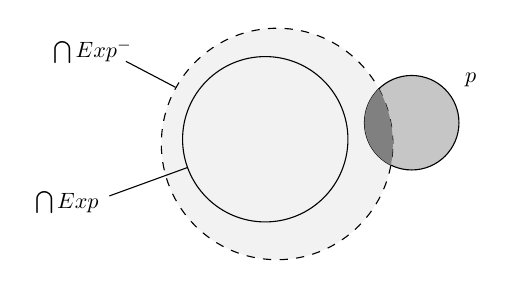
\begin{tikzpicture}[thick,scale=0.30, every node/.style={scale=0.80}]
%\def\ellipseP{[rotate=0](8,3.4) ellipse (2.3cm and 1.5cm)}
\def\ellipseP{(7.9,2.9) circle (2cm)}
\def\cercleExp{(1.7,2.2) circle (3.5cm)}
\def\cercleExpMoins{(2.2,2) circle (4.9cm)}
%
\fill[gray!10] \cercleExpMoins;
\draw[black, thin,fill=gray!45] \ellipseP;
\draw[black, thin] \cercleExp;
\draw[black, dashed, thin] \cercleExpMoins;
\begin{scope}
  \clip \cercleExpMoins;
  \fill [gray] \ellipseP;
\end{scope}
%
% Etiquettes :
\draw (10.4,4.7) node {$p$};
\draw[thin] (-1.6,1) -- (-4.9,-0.2);
\draw (-6.7,-0.5) node {$\bigcap Exp$};
\draw[thin] (-2.1,4.4) -- (-4.2,5.5);
\draw (-5.6,5.9) node {$\bigcap Exp^{-}$};
\end{tikzpicture}
\end{figure}

Moreover, the speaker may entertain different expectations about the truth of the prejacent, which lead to different expectation sets. For instance, imagine a situation where John leaves a meeting before it is finished. The speaker may consider this behaviour unacceptable on the basis of the rules. But she also may consider it unusual regarding John's habits. These two judgements correspond to two expectation sets, one about rules (Exp in Figure \ref{fig:fleury:2Exp}) and one about habits (Exp$_1$).

\begin{figure}
\caption{Two expectation sets}
\label{fig:fleury:2Exp}
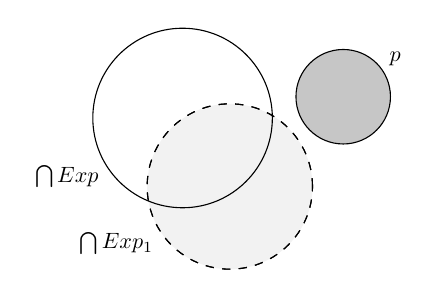
\begin{tikzpicture}[thick,scale=0.30, every node/.style={scale=0.80}]
%\def\ellipseP{[rotate=0](8.6,3.4) ellipse (2.3cm and 1.5cm)}
\def\ellipseP{(8.8,3.1) circle (2cm)}
\def\cercleExp{(2,2.2) circle (3.8cm)}
\def\cercleExpUn{(4,-0.7) circle (3.5cm)}
%
\draw[black, dashed, thin, fill=gray!10] \cercleExpUn;
%
\draw[rotate=0, black,fill=gray!45, thin] \ellipseP;%(8.3,1.5) ellipse (2.3cm and 1.5cm);
\draw (11,4.7) node {$p$};
%
%\filldraw[gray, thin] (3,3.3) circle (1cm);
%\draw[black, thin] (3,3.3) circle (1cm);
%\draw (2.3,2.2) node {$\mathcal{N}$};
%
\draw[black, thin] \cercleExp;%(2,2.2) circle (3.8cm);
\draw (-2.9,-0.3) node {$\bigcap Exp$};
%
\draw[black, dashed, thin] \cercleExpUn;
%
\draw (-0.8,-3.1) node {$\bigcap Exp_1$};
\end{tikzpicture}
\end{figure}

Neither the intersection of Exp 
nor that of Exp$_1$ intersect~$p$ in  Figure \ref{fig:fleury:2Exp}.
When the speaker asks the question \textit{comment peut-il quitter la r\'eunion avant la fin\,?} (how can he leave the meeting before the end?), 
she has some expectations incompatible with the prejacent~$p$.
But she may have different judgements corresponding to different expectations sets at the same time, that are incompatible with the prejacent $p$. What is crucial  is our assumption that a question is associated with one and only one {contextually relevant} expectation set.


%\ajout{
The propositions of Exp partitions the possible worlds into separate 
cells in a standard way.\footnote{For each cell, the propositions in Exp have the same truth values in all the worlds of the cell, the cells do not overlap, and cover all the possible worlds.} $\bigcap Exp$ is clearly one of the cells of the partition, namely the set of worlds where all the propositions in Exp are true.
%}


Now we want to define more precisely this partition and look at the information available to the speaker (her expectations, {the prejacent,} the new information) in terms of that partition. We are going to present the link between contingency and partition, and sketch the forms of modification the new information leads~to.


%%%%%%%%%%%%%%%%%%%%%%%%%%%%%%%%%%%%%%%%%%%%%%%%%%%%%%%%%%%%%%%%%%%%%%%%%%%%%%
\subsection{Subject matter and issues}\label{sec:fleury:subjectMatter}%{name=subject,column=2,below=high}{
%%%%%%%%%%%%%%%%%%%%%%%%%%%%%%%%%%%%%%%%%%%%%%%%%%%%%%%%%%%%%%%%%%%%%%%%%%%%%%
The notion of contingency is modelled by the non equivalence among possible worlds, so we need a way to compute equivalence classes among worlds.
%}
Two worlds are considered {alike} if the relevant propositions have the same truth values on these two worlds  \citep{Lewis88}. %(Lewis 1988).
This being alike is an {equivalence relation} that Lewis called 
\textit{subject matter}.
The equivalence classes of such a relation are the cells of a {partition} on the possible worlds $W$.
Each of its cells 
is a maximally specific way things might be with respect to relevant propositions. 
Intuitively, 
the minimal collection of relevant expectations can be seen as a thematic way to select worlds as a function of the expectations they are consistent with. 

In example (\ref{ex:fleury:Reason0}),
repeated in (\ref{ex:fleury:ReasonIssue0}), the relevant propositions are \textit{Max is respectful} ($p_1$) and \textit{if Max is respectful then he doesn't read the mail of others} (and specifically Paul's) ($p_1 \rightarrow \neg p$).
\begin{exe}
\ex\label{ex:fleury:ReasonIssue0}
\begin{xlist}
  \ex\label{ex:fleury:ReasonIssue1} Comment Max lit le courrier de Paul\,?\\
  How (is it/could it be) that Max read Paul's mail?
  \ex\label{ex:fleury:ReasonIssue2} Il est curieux (He is nosy)
  \ex\label{ex:fleury:ReasonIssue3} Max n'est pas respectueux (Max is not respectful)
\end{xlist}
\end{exe}

Assume {S\capsub{ex:fleury:p}}  is the subject matter that corresponds to the propositions in the expectation set {ex:fleury:p $=\{p_1,~p_1 \rightarrow \neg p\}$}.
The proposition $p_1$ is represented by the hatched area in Figure \ref{fig:fleury:notAnIssue}, and the proposition $(p_1 \rightarrow \neg p)$ by the grey area.\footnote{
By definition, $a\rightarrow{}b$ is equivalent to $\neg a \lor b$. Then the proposition $p_1\rightarrow \neg{}p$ is equivalent to $\neg p_1 \lor \neg p$ and also to $\neg(p_1 \land p)$. It corresponds to the grey area in Figure \ref{fig:fleury:notAnIssue}.}
The cells of the partition induced by these two propositions (i.e. the equivalence classes of S\capsub{ex:fleury:p}) are delimited by thick lines. The partition contains the cells $p \land p_1$ (white hatched area), $\neg p_1$ (non-hatched grey area) and $\neg p \land p_1$ (grey hatched area), i.e. all the combinations of the two relevant propositions $p_1$ and $(p_1\rightarrow \neg p)$, by using the logical connectives $\neg$ and~$\land$. There are only three cells in this example, because $\neg p_1 \land \neg (p_1\rightarrow \neg p)$ is empty for logical reasons.\footnote{The intersection of $\neg p_1$ (non-hatched grey area in Figure \ref{fig:fleury:notAnIssue}) and $\neg (p_1\rightarrow \neg p)$ (white hatched area) is empty.} 

\begin{figure}
\caption{S\capsub{ex:fleury:p}$[q] \neq$ S\capsub{ex:fleury:p}} 
\label{fig:fleury:notAnIssue}
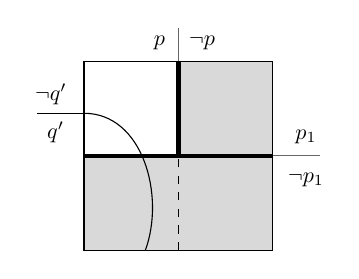
\begin{tikzpicture}[thick,scale=0.60, every node/.style={scale=0.80}]
%
%comment out the previous size command to enlarge the picture
%
\newcommand{\A}{(0,0)  coordinate (departA) -- ++(0,2) -- ++(2,0) -- ++(0,2) -- ++(2,0) -- ++(0,-4) -- cycle};
\newcommand{\B}{(0,2)  coordinate (departB) -- ++(0,2) -- ++(4,0) -- ++(0,-2) -- cycle};
\newcommand{\D}{(0,0) coordinate (departF) -- ++(0,2) -- ++(4,0) -- ++(0,-2) -- cycle};
%
% Cadre extérieur :
\draw[black,thin] (0,0) rectangle (4,4) ;
%
% Zone grise :
\draw[black,thin, fill=black!15, rounded corners=0pt, opacity=1] \A;
%
% Zone hachurée :
\hachure{0}{2}{2}{4}{1}{6}{thin}{black}{80};
\hachure{2}{2}{4}{4}{1}{6}{thin}{black}{80};
%\draw[black,thin,
%    pattern=north east hatch,hatch distance=5pt,hatch thickness=0.4pt,pattern color=black!70,
%   rounded corners=0pt, opacity=1] \B ;
%
\draw[thin,dashed,black] (2,0) -- (2,4);
%
%Etiquettes :
\draw[thin,black!60] (4,2) -- (5,2);
\draw[thin,black!60] (2,4) -- (2,4.7);
\draw (1.6,4.4) node {$p$};
\draw (2.5,4.4) node {$\neg p$};
\draw (4.7,2.4) node {$p_1$};
\draw (4.7,1.5) node {$\neg p_1$};
%
%Partition :
\draw[black, line width=1.5pt] (0,2) -- (4,2);
\draw[black, line width=1.5pt] (2,2) -- (2,4);
%
%Courbe + étiquettes :
\draw[thin,black] (0,2.9) to[out=0,in=70] (1.3,0);
\draw[thin,black] (0,2.9) -- (-1,2.9);
\draw[black] (-0.7,3.3) node {$\neg q'$};
\draw[black] (-0.6,2.5) node {$q'$};
\end{tikzpicture}
\end{figure}


%{\normalsize
A proposition {$q$} is considered an %\textbf{\textit{issue}}
\textit{issue} in the subject matter {S\capsub{ex:fleury:p}} iff {S\capsub{ex:fleury:p}$[q]=$ S\capsub{ex:fleury:p}}, where {S\capsub{ex:fleury:p}$[q]$} is the subject matter based on the proposition of Exp and {$q$}
\citep{fintelGillies10}.
In plain words, a proposition is an issue in a subject matter when its informative contribution is already taken into account in the computation of the partition.


Issues in S\capsub{ex:fleury:p} are non-contingent on each equivalence class of the subject matter S\capsub{ex:fleury:p}. In particular, $p_1$ and  $p_1 \rightarrow \neg p$ are issues in S\capsub{ex:fleury:p}.\footnote{Propositions $p_1$ and $p_1\rightarrow \neg{}p$ are not the only issues in the subject matter. For instance, $p \lor \neg p_1$ is also an issue. It is easy to verify that $p \lor \neg p_1$ is non-contingent on each cell of the partition: $p \lor \neg p_1$ is true on $p \land p_1$, true on $\neg p_1$, and false on $\neg p \land p_1$.
{Moreover, each proposition that corresponds to a cell is an issue, for it is true on the cell and false on the other cells (for the cells are non-overlapping). Likewise, the proposition that corresponds to the entire logical space is true on every cell and hence is an issue.}
}
By contrast, the proposition $q'$, as represented by a curved line in Figure~\ref{fig:fleury:notAnIssue}, is not an issue in the subject matter S\capsub{ex:fleury:p}, for the cell $p \land p_1$ contains both $q'$-worlds and $\neg q'$-worlds, 
and the same applies to the cell $\neg p_1$. In other words, the proposition $q'$ is contingent on the cells $p \land p_1$ and $\neg p_1$, and we have S\capsub{ex:fleury:p}$[q']~\neq$~S\capsub{ex:fleury:p}, more precisely: S\capsub{ex:fleury:p}$[q']=\{p \land p_1 \land q, \ p \land p_1 \land \neg q, \ \neg p_1 \land q, \ \neg p_1 \land \neg q, \ \neg p \land p_1\}$.

We will say that the expectation set is \textit{trivial} with respect to the prejacent $p$ if $p$ is a combination
%\footnote{} 
of the propositions in the expectation set. In order to clarify the notion of combination that we use, let us give an example with three propositions $p_1$, $p_2$ and $p_3$. The proposition $(p_1 \land p_2 \land \neg p_3) \lor (p_1 \land \neg p_2 \land p_3) \lor (p_1 \land \neg p_2 \land \neg p_3)$ is one of the combinations of the propositions $p_1$, $p_2$ and $p_3$.

In  example (\ref{ex:fleury:TrivialExp1}), the prejacent $p$ is \textit{Max va au cinema} (Max go to the cinema). Suppose the speaker thinks that a world where Max go to the cinema is not possible under any circumstances, and that there is no particular reason for that. 
In this case, the expectation set is simply $\{\neg p\}$ and $p$ is clearly a combination of the only proposition in the expectation set. 
The expectation set is trivial with respect to the prejacent and the question in (\ref{ex:fleury:TrivialExp1}) is not very natural.
\begin{exe}
\ex\label{ex:fleury:TrivialExp1} \gll Comment Max peut-il aller au cin\'ema\,?\\
how Max can-he go to-the cinema\\
\glt How can Max go to the cinema?
\end{exe}
Usually, what the speaker thinks about the truth or the possibility of~$p$ relies on some kind of reasoning about circumstances, rules, norms or regularities. For instance, Max is not used to going to the cinema or Max has to finish a book. In this case, the prejacent $p$ is not just a simple combination of the propositions in the expectation set.
Here, we suppose the expectation is not trivial with respect to the prejacent.
Then the prejacent cannot be an {issue} in the subject matter S\capsub{ex:fleury:p},
for an issue in the subject matter S\capsub{ex:fleury:p} is a combination of propositions in Exp.
In example (\ref{ex:fleury:ReasonIssue0}), it can be easily seen that the prejacent is contingent in some equivalence classes ($\neg p_1$), but non-contingent in some others (true in $p \land p_1$ and false in $\neg p \land p_1$). 
So the prejacent $p$ is not an issue in the subject matter S\capsub{ex:fleury:p}.

However, the expectations
of the speaker correspond to the cell $\neg p \land p_1$ (the intersection of Exp) where 
{the prejacent is non-contingently false}.
 This is why the speaker is stuck, and by asking a reason question with \textit{comment}, she aims at
undoing the status of non-contingency of the prejacent
in her expectations. Moreover, a relevant answer may or may not be an issue.


\section{Solving the conflict }\label{sec:fleury:spareBits}

\subsection{Congruent answers}\label{sec:fleury:conguent}

We have seen that by asking a reason question with \textit{comment}, the speaker aims at
undoing the non-contingent status of the prejacent
in her expectations. 
As mentioned in section 
\ref{sec:fleury:expSet}, this type of question  does not give rise to alternatives per se, contra canonical wh-questions.
What is a congruent answer cannot be stated in a standard manner
%}
\citep{Stechow91}.
Yet, it is not the case that anything will do for an answer. In this section we explore a way to characterise good answers.

To simplify things a bit, we suppose that the speaker's knowledge and belief belong to the common ground, i.e. the propositions shared by her and the addressee.
%}
The expectation set Exp of the speaker may include 
knowledge, belief and other judgements compatible with her knowledge and belief. Typically, these compatible judgements could be default judgements.  
They correspond to default rules that the speaker holds because of partly known information
\citep{Veltman96,CrespoKarawaniVeltman18}.\footnote{\citet[269]{CrespoKarawaniVeltman18} remind us that: 'Default rules are of crucial importance when some decision must be made in circumstances where the facts of the matter are only partly known. They affect an agent's expectations and as such help to narrow down the range of possibilities an agent has to take into account'.}
%
Moreover, they are not necessarily compatible with the addressee's knowledge and beliefs.
%}
The speaker is looking for some new information $q$
compatible with her knowledge and beliefs,
%}
such that  recomputing the expectation set with $q$ (Exp') makes the prejacent contingent, i.e. there exists a possible world compatible with Exp' where $q$ and the prejacent $p$ are true.



The expectation set Exp
partitions the possible worlds and, as seen in \sectref{sec:fleury:subjectMatter}, the new piece of information $q$ may or may not be an issue with respect to this partition, and thus leads to different possible modifications of the expectation set. The purpose of this partition is to distinguish
different kinds of modifications of the expectation set, not to represent the answers of the question.

When the speaker regards the answer $q$  as relevant, she modifies her expectations Exp according to this new information.
More precisely, the proposition $q$ is in a kind of conflit with at least one proposition in Exp, say~$p'$ (otherwise the speaker does not need to modify her expectations). If $q$ is an issue in the partition generated by Exp,
typically when $q$ is the negation of~$p'$,
then the speaker
may revise Exp by replacing $p'$ by $q$ in it.
In Paul's mail example, if $q$ is the information that Max is not respectful, that is $q = \neg p_1$, then
the speaker may replace $p_1$ by
$\neg p_1$ in her expectations. By contrast, if $q$ is not an issue, then she may replace $p'$ by a proposition compatible with some possible worlds that are both $q$ and $\neg p'$, while not necessarily considering the proposition $q$ as true.
%\ajout{
In Paul's mail example, if $q$ is the information that Max is nosy, then the speaker may consider that this information clashes to some extent with her expectation that Max is respectful ($p_1$). Indeed, the more someone is nosy ($q$), the more he or she is likely to be disrespectful ($\neg p_1$). This is not an implication between the fact that Max is nosy ($q$) and the fact that Max is disrespectful ($\neg p_1$). Nevertheless, it is commonly accepted -- under some general and shared principles -- that curiosity may lead to disrespect, in some circumstances. As a result, the speaker may accept the possibility that some $q$-worlds are also $\neg p_1$-worlds, without rejecting $\neg q$-worlds.
Let's note Exp' these new expectations.
If the speaker accepts the truth or the possibility of the proposition $q$, and if~$p$ is contingent in the new expectations Exp', i.e. $\bigcap Exp'$ intersects~$p$, then the proposition $q$ is a good answer.  %}
Moreover, if she considers the proposition $q$ true (not only possible), such a proposition 
%$q$ 
is added 
{to the previous expectation set Exp'. The new expectation set, i.e.  Exp''=Exp'$\cup \{q\}$, intersects $p$ as well.}
%
But if the speaker rejects the truth of $q$, then the proposition $\neg q$ is added to the expectation set Exp',
{and the new expectation set Exp'''= Exp'$\cup \{\neg q\}$ does not intersect $p$.}
The prejacent remains non-contigent and false with respect to  Exp'''. The proposition $q$ is a bad answer.


The modifications the answer $q$ may cause on the expectation set differ depending on whether the answer is an outcome or not. We look at this distinction with an in-depth discussion of an example in  \sectref{sec:fleury:issueNotIssue}.

%%%%%%%%%%%%%%%%%%%%%%%%%%%%%%%%%%%%%%%%%%%%%%%%%%%%%%%%%%%%%%%%%%%%%%%%%%%%%%
\subsection{Computing the expectation set}\label{sec:fleury:issueNotIssue}
%%%%%%%%%%%%%%%%%%%%%%%%%%%%%%%%%%%%%%%%%%%%%%%%%%%%%%%%%%%%%%%%%%%%%%%%%%%%%%
Relevant answers provide information that alters the non-contingent status of the prejacent, whether or not they are an issue in the subject matter.
Recall that, roughly speaking, a proposition is an issue in the subject matter if its informative  contribution is already taken into account.



\subsubsection{Getting new information that is an issue}

Assume question \textit{Comment Max lit le courrier de Paul\,?} in %(\ref{ex:fleury:Reason1})
(\ref{ex:fleury:ReasonIssue1}) gets the answer %(\ref{ex:fleury:ReasonIssue}). 
\textit{Max is not respectful} (\ref{ex:fleury:ReasonIssue3}). % (=(8)).
This answer  $\neg p_1$ is the negation of an expected proposition, and is an issue in the subject matter.
\begin{figure}
\caption{ex:fleury:p'}
\label{fig:fleury:issue}
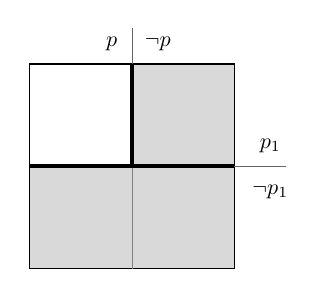
\begin{tikzpicture}[thick,scale=0.65, every node/.style={scale=0.80}]
%
\newcommand{\A}{(0,0)  coordinate (departA) -- ++(0,2) -- ++(2,0) -- ++(0,2) -- ++(2,0) -- ++(0,-4) -- cycle};
\newcommand{\B}{(0,2)  coordinate (departB) -- ++(0,2) -- ++(4,0) -- ++(0,-2) -- cycle};
\newcommand{\D}{(0,0) coordinate (departF) -- ++(0,2) -- ++(4,0) -- ++(0,-2) -- cycle};
%
% Cadre extérieur :
\draw[black,thin] (0,0) rectangle (4,4) ;
%
% Zone grise :
\draw[black,thin, fill=black!15, rounded corners=0pt, opacity=1] \A;
%
% Zone hachurée :
\hachure{0}{0}{2}{2}{1}{6}{thin}{black}{80};
\hachure{2}{0}{4}{2}{1}{6}{thin}{black}{80};
%\draw[black,thin,
%    pattern=north east hatch,hatch distance=5pt,hatch thickness=0.4pt,pattern color=black!70,
%   rounded corners=0pt, opacity=1] \D ;
%
% Proposition p :
\draw[thin,black!50] (2,0) -- (2,4);
%
%Etiquettes :
\draw[thin,black!60] (4,2) -- (5,2);
\draw[thin,black!60] (2,4) -- (2,4.7);
\draw (1.6,4.4) node {$p$};
\draw (2.5,4.4) node {$\neg p$};
\draw (4.7,2.4) node {$p_1$};
\draw (4.7,1.5) node {$\neg p_1$};
%
%Partition :
\draw[black, line width=1.5pt] (0,2) -- (4,2);
\draw[black, line width=1.5pt] (2,2) -- (2,4);
%
\end{tikzpicture}
\end{figure}

If the speaker accepts answer $\neg p_1$, the subject matter is unchanged,
% -- the lower half of the drawing -- 
but the new expectation set is
%\\
Exp'=$\{\neg p_1,~p_1\rightarrow{}\neg p\}$
%\\
and the possible worlds are
%\\
\mbox{$\bigcap$ Exp'=} $\neg p_1$
%}
%\\
%cf. green hatched lower half area.%}
(grey hathed lower half area in Figure \ref{fig:fleury:issue}).
The proposition $p$ becomes contingent in the expectation set Exp' and
%\sout{$q$}
%\ajout{
$\neg p_1$
%}
is a good answer.



\subsubsection{Getting new information that is not an issue}


Consider question 
(\ref{ex:fleury:ReasonIssue1}), and the possible answer \textit{Max est trop curieux} 
(Max is way too nosy) ($q$).
Proposition $q$ is not an issue in S\capsub{ex:fleury:p},
for it is contingent in at least one cell of the partition. Among the worlds where Max is respectful and does not read Paul's mail ($p_1 \land \neg p$), we can imagine some possible worlds where 
Max is nosy
(but not to the point that he reads Paul's mail), and others
where 
he is not nosy at all. In other words, the proposition $q$ is contingent in the cell $p_1 \land \neg p$.
%
If the speaker judges it relevant, it may be taken as a {possible cause} for the lack of respect by Max ($\neg p_1$), but does not entail it.
In other worlds, among $q$-worlds 
(worlds where Max is nosy), $p_1$-worlds as well as $\neg p_1$-worlds seem possible to the speaker 
(Max may or may not be disrespectful when he is nosy).
But $\neg q$-worlds are still expected to be $p_1$-worlds. So $\neg q\rightarrow p_1$ is expected. Moreover, the proposition $p_1\rightarrow \neg p$ is still expected (if Max is respectful, he does not read Paul's mail). The new expectation set is Exp''=$\{\neg q\rightarrow p_1,~p_1\rightarrow \neg p\}$, that is $(q \land \neg p_1) \lor (p_1 \land \neg p)$.\footnote{
Visually, the intersection of $\neg q\rightarrow p_1$ (hatched area) and $p_1\rightarrow \neg p$ (grey area) corresponds to the grey hatched area in Figure \ref{fig:fleury:pContingent}, that is the union of the top right squarre ($p_1 \land \neg p$) and the bottom half of $q$ (i.e. $q \land \neg p_1$). We can also calculate it as follows :
\\$(\neg q\rightarrow p_1) \land (p_1\rightarrow \neg p)$
\\$= (q \lor p_1) \land (\neg p_1 \lor \neg p)$
\\$= (q \land \neg p_1) \lor (q \land \neg p) \lor (p_1 \land \neg p_1) \lor (p_1 \land \neg p)$
\\$= (q \land \neg p_1) \lor (q \land \neg p) \lor (p_1 \land \neg p)$
\\$= (q \land \neg p_1) \lor ((q \land \neg p \land \neg p_1) \lor (q \land \neg p \land p_1)) \lor (p_1 \land \neg p)$
\\$= ((q \land \neg p_1) \lor (q \land \neg p \land \neg p_1)) \lor ((q \land \neg p \land p_1) \lor (p_1 \land \neg p))$
\\$= (q \land \neg p_1) \lor (p_1 \land \neg p)$
\\for $q \land \neg p \land \neg p_1 \subseteq q \land \neg p_1$ and $q \land \neg p \land p_1 \subseteq p_1 \land \neg p$.}

\begin{figure}
\caption{ex:fleury:p''}
\label{fig:fleury:pContingent}
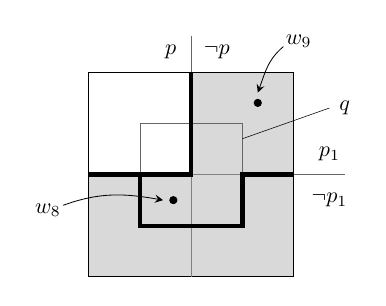
\begin{tikzpicture}[thick,scale=0.65, every node/.style={scale=0.80}]
\newcommand{\A}{(0,0)  coordinate (departA) -- ++(0,2) -- ++(2,0) -- ++(0,2) -- ++(2,0) -- ++(0,-4) -- cycle};
\newcommand{\B}{(0,2)  coordinate (departB) -- ++(0,2) -- ++(4,0) -- ++(0,-2) -- cycle};
\newcommand{\D}{(0,0) coordinate (departF) -- ++(0,2) -- ++(4,0) -- ++(0,-2) -- cycle};
%
% Cadre extérieur :
\draw[black,thin] (0,0) rectangle (4,4) ;
%
% Zone grise :
\draw[black,thin, fill=black!15, rounded corners=0pt, opacity=1] \A;
%
%Coloriage et hachurage :
%\fill[black!35] (0,0) rectangle (4,2);
%\fill[black!35] (2,2) rectangle (4,4);
\hachure{0}{2}{2}{4}{1}{6}{thin}{black}{80};
\hachure{2}{2}{4}{4}{1}{6}{thin}{black}{80};
\hachure{1}{1}{2}{2}{1}{3}{thin}{black}{80};
\hachure{2}{1}{3}{2}{1}{3}{thin}{black}{80};
%
% Proposition p :
\draw[thin,black!50] (2,0) -- (2,4);
% Proposition q :
\draw[thin,black!60] (1,1) rectangle (3,3);  
% Proposition p1 :
\draw[thin,black!50] (2,2) -- (4,2); 
%
%Etiquettes :
\draw[thin,black!60] (4,2) -- (5,2);
\draw[thin,black!60] (2,4) -- (2,4.7);
\draw (1.6,4.4) node {$p$};
\draw (2.5,4.4) node {$\neg p$};
\draw (4.7,2.4) node {$p_1$};
\draw (4.7,1.5) node {$\neg p_1$};
\draw[black,very thin] (3,2.7) -- (4.7,3.3);
\draw (5.0,3.3) node {$q$};
%
%Partition :
\draw[black, line width=1.5pt] (0,2) -- (2,2) -- (2,4);
\draw[black, line width=1.5pt] (0,2) -- (1,2) -- (1,1) -- (3,1) -- (3,2) -- (4,2);
%
%Points :
\fill[black] (1.65,1.5) circle (0.08cm);
\draw[black, line width=0.3pt, ->,>=stealth] (-0.5,1.4) to[out=20,in=170] (1.45,1.5);
\draw[black] (-0.8,1.3) node {$w_8$};
%
\fill[black] (3.3,3.4) circle (0.08cm);
\draw[black, line width=0.3pt, ->,>=stealth] (3.8,4.5) to[out=-140,in=70] (3.3,3.6);
\draw[black] (4.1,4.6) node {$w_9$};
\end{tikzpicture}
\end{figure}

Then,
the prejacent $p$ is contingent in the intersection of the new expectation set Exp'' (grey hatched area in Figure~\ref{fig:fleury:pContingent}). Either $\neg p$-worlds ($w_9$ in Figure~\ref{fig:fleury:pContingent}), or $p$-worlds ($w_8$ in Figure~\ref{fig:fleury:pContingent}), are possible worlds with respect to this new expectation set. Thus, $q$ is a good answer.

At this point, we have to distinguish two cases, the case where the new piece of information is deemed to be false, and the case where it is deemed to be true.
Let's start by the case where  the speaker does not accept the truth of answer $q$.
The new expectation set is
Exp''' = $\{\neg q\rightarrow p_1,~ p_1\rightarrow \neg p,~\neg q\}$
and the possible worlds are
$\bigcap$~Exp''' = $\neg p \land p_1 \land \neg q$
(cf. the grey hatched area in Figure \ref{fig:fleury:pContingentNotAcceptp3}).
The proposition $p$ remains non-contingent and false in the expectation set Exp''', i.e. $q$ is not a good answer.

\begin{figure}
\captionof{figure}{ex:fleury:p'''}
\label{fig:fleury:pContingentNotAcceptp3}
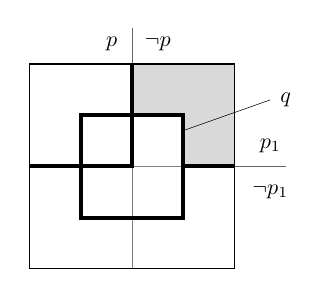
\begin{tikzpicture}[thick,scale=0.65, every node/.style={scale=0.80}]
%Coloriage et hachurage :
\fill[black!15] (2,3) rectangle (4,4);
\fill[black!15] (3,2) rectangle (4,3);
\hachure{2}{3}{3}{4}{1}{3}{thin}{black}{80};
\hachure{3}{3}{4}{4}{1}{3}{thin}{black}{80};
\hachure{3}{2}{4}{3}{1}{3}{thin}{black}{80};
%\hachure{2}{1}{3}{2}{1}{4}{thin}{black}{80};
%\fill[black!50] (2,3) rectangle (4,4);
%\fill[black!50] (3,2) rectangle (4,3);
%
% Proposition p :
\draw[thin,black!50] (2,0) -- (2,4);
% Proposition p1 :
\draw[thin,black!50] (2,2) -- (4,2);
%
%Quadrillage :
%\draw[thin,black!60] \foreach \p in {0,...,2} {(0,\p*2)--(4,\p*2) (\p*2,0)--(\p*2,4)};
\draw[thin,black!60] (4,2) -- (5,2);
\draw[thin,black!60] (2,4) -- (2,4.7);
\draw[thin,black!60] (1,1) rectangle (3,3);  
%
%Etiquettes :
\draw[thin,black!60] (4,2) -- (5,2);
\draw[thin,black!60] (2,4) -- (2,4.7);
\draw (1.6,4.4) node {$p$};
\draw (2.5,4.4) node {$\neg p$};
\draw (4.7,2.4) node {$p_1$};
\draw (4.7,1.5) node {$\neg p_1$};
\draw[black,very thin] (3,2.7) -- (4.7,3.3);
\draw (5.0,3.3) node {$q$};
%
%Partition :
\draw[black, line width=1.5pt] (0,2) -- (2,2) -- (2,4);
%\draw[black, line width=1.5pt] (0,2) -- (1,2) -- (1,1) -- (3,1) -- (3,2) -- (4,2);
\draw[black, line width=1.5pt] (1,3) -- (1,1) -- (3,1) -- (3,3) -- (1,3) -- (1,1);
\draw[black, line width=1.5pt] (3,2) -- (4,2);
%
% Cadre extérieur :
\draw[black,thin] (0,0) rectangle (4,4) ;
\end{tikzpicture}
\end{figure}

Now assume the speaker accepts the truth of answer~$q$. The
new expectation set is
Exp'''' = $\{\neg q\rightarrow p_1,~ p_1\rightarrow \neg p,~q\}$
and the possible worlds are
$\bigcap$ Exp'''' = $(q \land \neg p_1) \lor (q \land \neg p)$
(the grey hatched area in Figure \ref{fig:fleury:pContingentAcceptp3}).
The proposition $p$ becomes contingent in the expectation set Exp'''', and $q$ is a good answer.

\begin{figure}
\caption{ex:fleury:p''''}
\label{fig:fleury:pContingentAcceptp3}
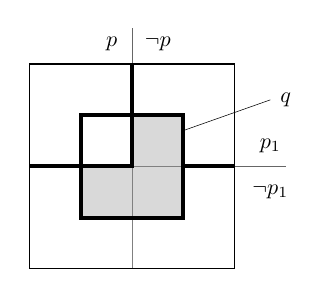
\begin{tikzpicture}[thick,scale=0.65, every node/.style={scale=0.80}]
%
%Coloriage et hachurage :
\fill[black!15] (1,1) rectangle (3,2);
\fill[black!15] (2,2) rectangle (3,3);
\hachure{1}{1}{2}{2}{1}{3}{thin}{black}{80};
\hachure{2}{1}{3}{2}{1}{3}{thin}{black}{80};
\hachure{2}{2}{3}{3}{1}{3}{thin}{black}{80};
%\hachure{2}{1}{3}{2}{1}{4}{thin}{black}{80};
%\fill[black!50] (1,1) rectangle (3,2);
%\fill[black!50] (2,2) rectangle (3,3);
%
% Proposition p :
\draw[thin,black!50] (2,0) -- (2,4);
% Proposition p1 :
\draw[thin,black!50] (2,2) -- (4,2);
%
%Etiquettes :
\draw[thin,black!60] (4,2) -- (5,2);
\draw[thin,black!60] (2,4) -- (2,4.7);
\draw (1.6,4.4) node {$p$};
\draw (2.5,4.4) node {$\neg p$};
\draw (4.7,2.4) node {$p_1$};
\draw (4.7,1.5) node {$\neg p_1$};
\draw[black,very thin] (3,2.7) -- (4.7,3.3);
\draw (5.0,3.3) node {$q$};
%
%Partition :
\draw[black, line width=1.5pt] (0,2) -- (2,2) -- (2,4);
%\draw[black, line width=1.5pt] (0,2) -- (1,2) -- (1,1) -- (3,1) -- (3,2) -- (4,2);
\draw[black, line width=1.5pt] (1,3) -- (1,1) -- (3,1) -- (3,3) -- (1,3) -- (1,1);
\draw[black, line width=1.5pt] (3,2) -- (4,2);
%
% Cadre extérieur :
\draw[black,thin] (0,0) rectangle (4,4) ;
\end{tikzpicture}
\end{figure}

Summing up, in this section,
we have seen that different statuses of the new information with respect to  the expectation set, i.e. its information contribution, lead to different modifications of the expectation set. New information that is not an issue leads the speaker to refine her default judgements, whereas new information that is an issue invites the speaker to negate some of her expectations. When this computation fails, the new information is not able to align the viewpoints of the interlocutors about preconditions to admitting the prejacent into the common ground.



\section{Concluding remarks}
\label{sec:fleury:conclusion}

This paper has explored further the hypothesis put forth by  \cite{FleuryTovena18} that
questions  with \textit{comment} in their reason reading 
primarily verbalise the  speaker's attempt to bounce back from an expectation disconfirmation, and convey her request for information that would count towards admitting the prejacent in the common ground. A host of empirical observations  motivate the adoption of a syntactic analysis for reason-\textit{comment} as merged high, a position from which it
can semantically operate on the speaker's expectations.\footnote{An analysis in terms of syntactic operator and no variable binding has been proposed for \textit{why} by \cite{StepanovTsai08}. More work is needed to assess if its suits reason-\textit{comment}.}

In these
questions, the sentence radical does not provide the alternatives corresponding to the congruent answers \textit{per se}. 
The information brought by a congruent answer allows the speaker to modify her expectations so as to undo the non-contingency of the prejacent. 
%\ajout{
In our analysis, the minimal collection of relevant expectations provides a thematic way to select worlds as a function of the expectations they are consistent with. The net result is that the expectations work like the modal base found in a kratzerian approach to modality, where 
the worlds that are faithful to the collection of propositions called modal base (epistemic, circumstantial) are selected and form a domain the modal quantifies over.
Note, however, that the partition of the worlds induced by the expectation set is not meant to represent the answers of the question, but to distinguish different kinds of modifications of the expectation set brought about by different answers.
An open research question is to explore  whether our solution can restore the possibility of an analysis of reason-\textit{comment} questions in terms of a quantifier binding a variable.
%}


The speaker's expectations are characterised as a minimal set of propositions that makes the prejacent false and non-contingent. Expectations partition the possible worlds in such a way that the prejacent is not an issue with respect to this partition. 
Congruent answers, which may or may not be issues, enable the speaker to recompute the partition by negating or refining her expectations.

Finally, our analysis allows us to account for a difference in the reason reading between \textit{comment} and \textit{why} so far unnoticed, to the best of our knowledge. Suppose a context where Paul and his friends know he has to stop drinking. He doesn't, and his friends discuss about the situation. The data in (\ref{ex:fleury:Fumer0}) show that  \textit{comment} and \textit{why} differ  with respect to their compatibility with an answer that provides an explanation with no causal relation to the event.
\begin{exe}
\ex \label{ex:fleury:Fumer0} 
\begin{xlist}
\ex \label{ex:fleury:Fumer1} \gll Q: Comment Paul continue \`a boire\,?
  A:   Il continue bien \`a fumer.\\
{} how  Paul continues to drink  {} he continues well to smoke \\
\glt How come Paul continues to drink? Well, he continues to smoke too.
\ex \label{ex:fleury:Fumer2} \gll Q: Pourquoi Paul continue \`a boire\,?
  A:   \#Il continue bien \`a fumer.\\
{} why  Paul continues to drink  {} he continues well to smoke \\
\glt Why does Paul continue to drink?  Well, he continues to smoke too.
\end{xlist}
\end{exe}

Our device authorises the answer provided in (\ref{ex:fleury:Fumer1}) to resolve the conflict.
In this example, the answer resolves the conflict in virtue of the general principle that if one does not follow a recommendation in one area, it is possible/probable/ not improbable that one will not follow a recommendation in a similar area. On the other hand, such an answer can hardly be regarded as a cause of the prejacent or even a reason corresponding to the similar question with \textit{pourquoi} presented in (\ref{ex:fleury:Fumer2}).


\printbibliography[heading=subbibliography,notkeyword=this]

\end{document}
